\documentclass[a4paper]{scrartcl}
\usepackage[utf8]{inputenc}
\usepackage{showframe} % disable this to hide #border.
\usepackage{wrapfig}
% Example:
% \begin{wrapfigure}{R}{0.4\textwidth}
% \centering
% 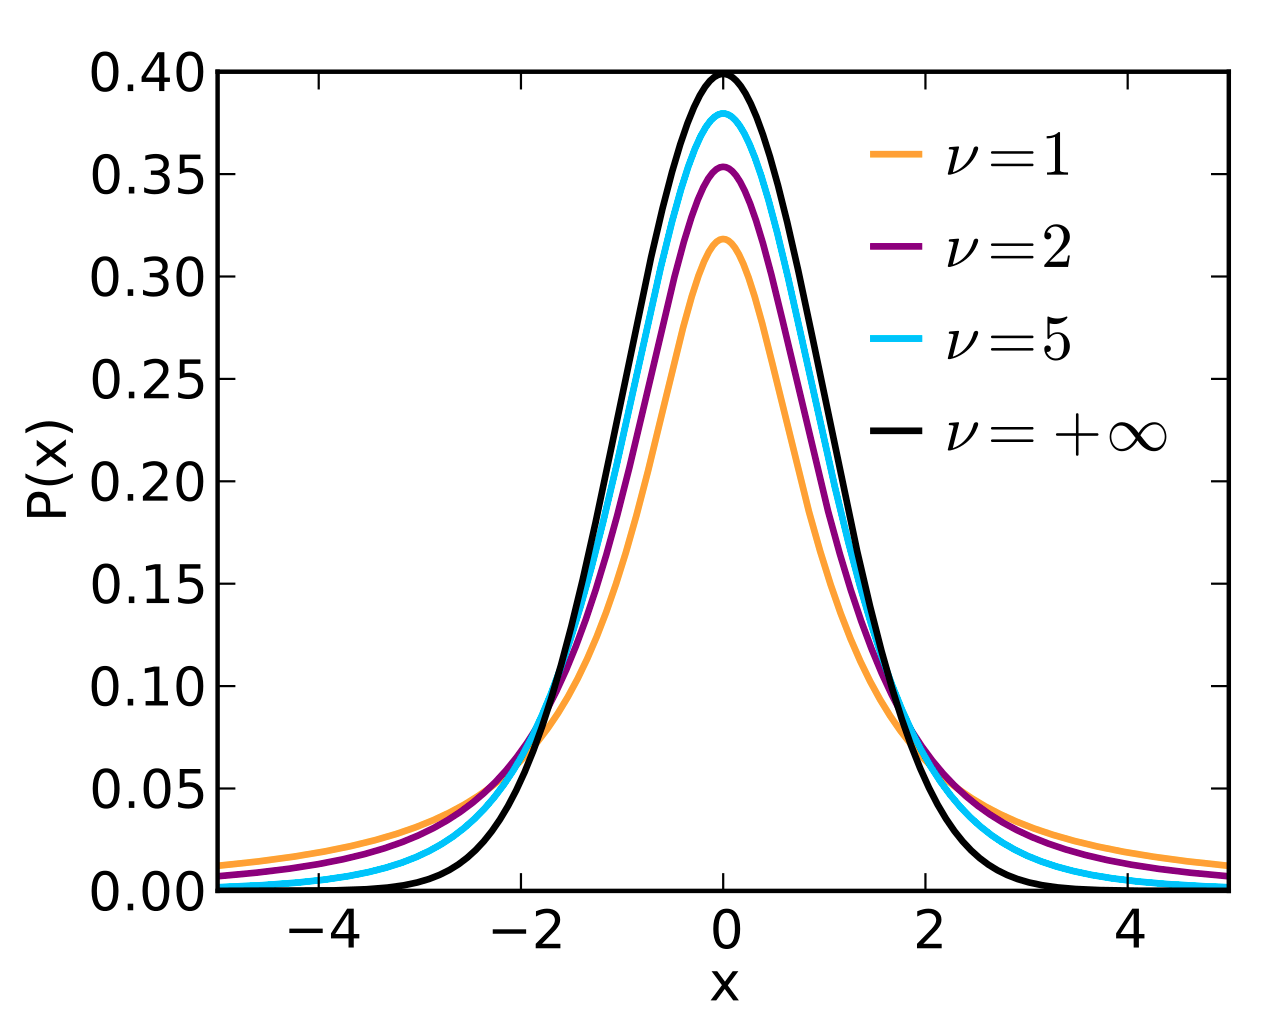
\includegraphics[width=0.35\textwidth]{assets/lectures_part_3-91d0349d.png}
% The PDF of the Student distribution.
% \end{wrapfigure}


\usepackage[english, russian, ukrainian]{babel}
\usepackage{misccorr,
            color,
            ragged2e,
            amsfonts,
            amsthm,
            graphicx,
            systeme,
            amsmath,
            mdframed,
            lipsum,
            mathtools,
            setspace
            }

\renewcommand\qedsymbol{$\blacksquare$}
\renewcommand*{\proofname}{\text{Доведення}}

\theoremstyle{definition}
\newtheorem*{defo}{Означення}
\newtheorem*{lemme}{Лема}
\newtheorem*{example}{Приклад}
\theoremstyle{remark}
\newtheorem*{remark}{Зауваження}
\theoremstyle{definition}
\newtheorem*{consequence}{Наслідок}
\theoremstyle{definition}
\newtheorem{statement}{Твердження}[section]
\newmdtheoremenv{boxteo}{Теорема}[section]

\setlength{\parindent}{0em}
\setlength{\parskip}{0.5em}
\DeclareMathOperator*\lowlim{\underline{lim}}
\DeclareMathOperator*\uplim{\overline{lim}}

\newcommand\independent{\protect\mathpalette{\protect\independenT}{\perp}}
\def\independenT#1#2{\mathrel{\rlap{$#1#2$}\mkern2mu{#1#2}}}

\usepackage{tikz}
\newcommand*\circled[1]{\tikz[baseline=(char.base)]{
  \node[shape=circle,draw,inner sep=1pt] (char) {#1};}}

% Default fixed font does not support bold face
\DeclareFixedFont{\ttb}{T1}{txtt}{bx}{n}{12} % for bold
\DeclareFixedFont{\ttm}{T1}{txtt}{m}{n}{12}  % for normal

% Custom colors
\definecolor{deepblue}{rgb}{0,0,0.5}
\definecolor{deepred}{rgb}{0.6,0,0}
\definecolor{deepgreen}{rgb}{0,0.5,0}

\usepackage{listings}

% Python style for highlighting
\newcommand\pythonstyle{\lstset{
language=Python,
basicstyle=\ttm,
morekeywords={self},              % Add keywords here
keywordstyle=\ttb\color{deepblue},
emph={MyClass,__init__},          % Custom highlighting
emphstyle=\ttb\color{deepred},    % Custom highlighting style
stringstyle=\color{deepgreen},
frame=tb,                         % Any extra options here
showstringspaces=false
}}


% Python environment
\lstnewenvironment{python}[1][]
{
\pythonstyle
\lstset{#1}
}
{}

% Python for external files
\newcommand\pythonexternal[2][]{{
\pythonstyle
\lstinputlisting[#1]{#2}}}

% Python for inline
\newcommand\pythoninline[1]{{\pythonstyle\lstinline!#1!}}

%                 USAGE:
% \begin{python}
% class MyClass(Yourclass):
%     def __init__(self, my, yours):
%         bla = '5 1 2 3 4'
%         print bla
% \end{python}
%
%
% \pythonexternal{demo.py}
%
%
% Definition \pythoninline{class MyClass} means \dots

\def\be{\begin{equation}}      % equation
\def\ee{\end{equation}}        % ...
\def\i{\infty}                 % infinity
\def\d{\partial}               % dx dy - partial     = \d
\def\bdash{\ \Big|\  }         % big vertical line   = |
\def\index{\mathbb{I}}         % indicator
\def\res#1{\underset{#1}{\mathrm{res}}}

\begin{document}
\tableofcontents
\newpage

\begin{center}
	\Huge \textbf{Ряд Фур'є}
\end{center}
\par
\section{Лекція 1.}
\subsection{Поява. Передмова.}
Нехай $g(z)$ -- аналітична в  кільці $K = \left\lbrace  z \bdash 1 - \varepsilon_1 < |z| < 1 + \varepsilon_2 \right\rbrace$; $ \left\lbrace  z \bdash  |z| = 1 \right\rbrace \subset K.$\par
Розкладаємо $g(z)$ в ряд Лорана за степенями $z $ в цьому кільці:
$$
g(z) =  \sum\limits_{n =  - \i}^{ \infty}{ C_n \cdot z^n} \text{ , де } C_n = \frac{1}{2\pi i}  \int\limits_{|z| = 1 }^{ }{ \frac{ g(z)}{z^{n+1} }  \mathrm{d} z}
$$
$$
z : |z| =1 \ \Longrightarrow \  z = e^{ix} \ \Longrightarrow \  x \in  [0, 2 \pi]
 \ \Longrightarrow \
g(z) = g(e^{ix}) = f(x)
$$
$$
C_n = \frac{1}{2\pi i}  \int\limits_{|z| = 1 }^{ }{ \frac{ g(z)}{z^{n+1} }  \mathrm{d} z} = \left|  \begin{gathered}
  z = e^{ix}\\
  \mathrm{d} z = ie^{ix} \mathrm{d} x \\
  x \in [0, 2\pi]
\end{gathered} \right| = \frac{1}{2\pi}  \int\limits_{0}^{ 2 \pi}{ f(x) e^{-inx} \mathrm{d} x}
$$
Отримали \textit{комплексну форму ряду Фур'є}:
$$
f(x) =  \sum\limits_{n =-\i }^{ \infty}{C_n \cdot e^{inx}}, \  C_n =  \frac{1}{2\pi}  \int\limits_{0}^{ 2 \pi}{ f(x) e^{-inx} \mathrm{d} x}
$$
\subsection{Комплексна форма ряду Фур'є.}

$f \in D[0, 2\pi]$ -- періодична, інтегрова на $[0, 2 \pi]$. За функцією $f(x)$ будуємо ряд Фур'є:
$$
S(x) =  \sum\limits_{n =-\i }^{ \infty}{C_n \cdot e^{inx}}, \  C_n =  \frac{1}{2\pi}  \int\limits_{0}^{ 2 \pi}{ f(x) e^{-inx} \mathrm{d} x}
$$
Питання:
\begin{enumerate}
  \item  Збіжність ряду.
\item  Якщо збігається, то зв'язок між $S(x)$ та $f(x)$.
\end{enumerate}
\subsection{Випадок дійснозначної функції.}
Розглянемо ряд Фур'є:
$$
 \sum\limits_{n = -\infty}^{ -1}{C_n \cdot e^{inx}} + C_0 +  \sum\limits_{n = 1}^{ \infty}{C_n e^{inx}} = \left| \begin{gathered}
  \text{в І сумі:}\\
  n= -k
 \end{gathered} \right| =  \sum\limits_{k = 1}^{ \infty}{C_{-k} \cdot e^{-ikx}} + C_0 +  \sum\limits_{n = 1}^{ \infty}{C_n e^{inx}} \ \circled{=}
$$
Окремо розглянемо $C_{-k} e^{-ikx}$: $C_{-k} e^{-ikx} = \overline{C_{k} e^{ikx}}$:
$$
\circled{=} \ C_0 +  \sum\limits_{n = 1}^{ \infty}{\underbrace{\left( C_n e^{inx} + \overline{C_n e^{inx}} \right)}_{ = 2 \Re(C_n e^{inx})\in \mathbb{R}}} \ \fbox{$=$}
$$
$$
C_n = \frac{1}{2\pi}  \int\limits_{0}^{ 2 \pi}{ f(x) e^{-inx} \mathrm{d} x} = \frac{1}{2 \pi}   \int\limits_{0}^{ 2 \pi}{ f(x) \cdot \left( \cos{(nx)} - i \sin{(nx)} \right) \mathrm{d} x} =
$$
$$
 = \frac{1}{2\pi} \int\limits_{0}^{ 2 \pi}{ f(x) \cdot  \cos{(nx)} \mathrm{d} x} - i\frac{1}{2\pi}  \int\limits_{0}^{ 2 \pi}{ f(x) \cdot  \sin{(nx)} \mathrm{d} x}
$$
$$
 \Re C_n e^{inx} \!=\! \Re \left[ \frac{1}{2\pi}\!\int\limits_{0}^{ 2 \pi}{ f(x)  \cos{(nx)} \mathrm{d} x} - i \frac{1}{2\pi}\! \int\limits_{0}^{ 2 \pi}{ f(x)  \sin{(nx)} \mathrm{d} x}  \right] \cdot \left( \cos{(nx)} + i \sin{(nx)} \right)\! =
$$
$$
= \frac{1}{2\pi} \cos{(nx)} \int\limits_{0}^{ 2 \pi}{ f(x) \cdot  \cos{(nx)} \mathrm{d} x} + \frac{1}{2\pi}\sin{(nx)}  \int\limits_{0}^{ 2 \pi}{ f(x) \cdot  \sin{(nx)} \mathrm{d} x}
$$
$$
\fbox{$=$} \  C_0 +  \frac{1}{\pi} \sum\limits_{n = 1}^{ \infty}{
 \cos{(nx)} \int\limits_{0}^{ 2 \pi}{ f(x) \cdot  \cos{(nx)} \mathrm{d} x} + \sin{(nx)}  \int\limits_{0}^{ 2 \pi}{ f(x) \cdot  \sin{(nx)} \mathrm{d} x}
}
$$
$$
 C_0 = \frac{1}{2\pi}  \int\limits_{0}^{2\pi}{ f(x)dx} \qquad \quad \text{ Отримали} \textit{ дійсну форму ряда Фур'є.}
$$
$$
f(x) \mapsto \frac{a_0}{2} +  \sum\limits_{n = 1 }^{ \infty}{a_n \cos{( nx)} + b_n \sin{(nx)}},
$$
де $
a_n = \frac{1}{\pi}  \int\limits_{0}^{ 2\pi}{f(x) \cos{(nx)} \mathrm{d} x} , n \in \mathbb{N}\cup \left\lbrace 0 \right\rbrace ; \  b_n = \frac{1}{\pi}  \int\limits_{0}^{ 2\pi}{f(x) \sin{(nx)} \mathrm{d} x}, n \in \mathbb{N}\cup \left\lbrace 0 \right\rbrace.
$
\newpage

\subsection{Не $2\pi$-періодичні функції.}
$f$  -- $2l$ періодична, або задана на $[0, 2l]$, інтегрована. Розглянемо відображення:
$$
[0, 2\pi] \leftarrow [0, 2l] \qquad x \in [0, 2\pi] \qquad x = \frac{t}{l}\pi \qquad t\in [0, 2\pi]
$$
Тоді $f(x) = f( \frac{t}{l}\pi ) = g(t)$. $g(t)$ - задана на $[0, 2\l]$.
$$
a_n = \frac{1}{\pi}  \int\limits_{0}^{2\pi}{ f(x) \cos{(nx)} \mathrm{d} x } =   \frac{1
}{l }  \int\limits_{0}^{2l}{ g(t) \cos{ \left( \frac{\pi n t}{l}  \right)} \mathrm{d} t}
$$
$$
b_n = \frac{1}{\pi}  \int\limits_{0}^{2\pi}{ f(x) \sin{(nx)} \mathrm{d} x } =   \frac{1
}{l }  \int\limits_{0}^{2l}{ g(t) \sin{ \left( \frac{\pi n t}{l}  \right)} \mathrm{d} t}
$$
$$
g(t) = f(x) \mapsto \frac{a_0}{2} +  \sum\limits_{n = 1}^{ \infty}{a_n \cos{ \left(  \frac{\pi n t}{l} + b_n\sin{ \left( \frac{\pi n t}{l}  \right)}   \right)}}
$$
$$
a_n =\frac{1
}{l }  \int\limits_{0}^{2l}{ g(t) \cos{ \left( \frac{\pi n t}{l}  \right)} \mathrm{d} t}
 \qquad b_n = \frac{1
}{l }  \int\limits_{0}^{2l}{ g(t) \sin{ \left( \frac{\pi n t}{l}  \right)} \mathrm{d} t}
$$
Частіше всього, зручно обчислювати коефіцієнти ряду інакше:
$$
a_n =\frac{1
}{l }  \int\limits_{-l}^{l}{ g(t) \cos{ \left( \frac{\pi n t}{l}  \right)} \mathrm{d} t}
 \qquad b_n = \frac{1
}{l }  \int\limits_{-l}^{l}{ g(t) \sin{ \left( \frac{\pi n t}{l}  \right)} \mathrm{d} t}
$$

\subsection{Аналіз збіжності ряду.}
\begin{lemme}[Рімана]
$f$ -- інтегрована на $[a,b]$ навіть в невласному сенсі. \par Тобто $ \int\limits_{a}^{b}{f(x) \mathrm{d} x}$ -- збігається. Тоді:
\begin{enumerate}
  \item $\displaystyle  \int\limits_{a}^{ b}{f(x) \cos{(\lambda x)} \mathrm{d} x } \xrightarrow[\lambda\to\infty]{} 0 $
    \item $\displaystyle  \int\limits_{a}^{ b}{f(x) \sin{(\lambda x)} \mathrm{d} x } \xrightarrow[\lambda\to\infty]{} 0 $
\end{enumerate}

\end{lemme}

\end{document}
